\subsection{Inleiding}
Dit is een handleiding geschreven als informatieve bron bij het gebruik van de website “Verkeer-4.vop.tiwi.be”. Het beoogt een overzicht te geven bij het opzoeken van verkeersinformatie in en rond Gent. Dit zowel realtime als in het verleden.

\subsection{Het Dashboard}
Bij het surfen naar “Verkeer-4.vop.tiwi.be” zal u verwezen worden naar het dashboard van de website. Hier kunt u een korte samenvatting vinden van de belangrijkste informatie rond verkeer. 

\begin{itemize}
\item \textbf{Status - Errors} geeft een overzicht van de recente gebeurtenissen rond de applicatie. Het geeft een beeld van wat er misloopt.
\item \textbf{POI Overview} biedt een overzicht van de huidige “Points Of Interest”.  Hier worden onder andere ongevallen, trajectcontroles en belangrijke evenementen aangehaald.
\item De \textbf{Minimap} zorgt voor een visuele weergave van de verkeersituatie in en rond Gent. Zowel de files als de POI’s worden weergeven.
\item De \textbf{Weather widget} wordt gebruikt om een korte schets van het weer in Gent te weergeven. Dit kan het verkeer namelijk sterk beïnvloeden.
\item De \textbf{Twitter Wall}  toont de recente gebeurtenissen in en rond Gent die werden gemeld door de stad Gent.
\end{itemize}

\begin{figure}[H]
\centering
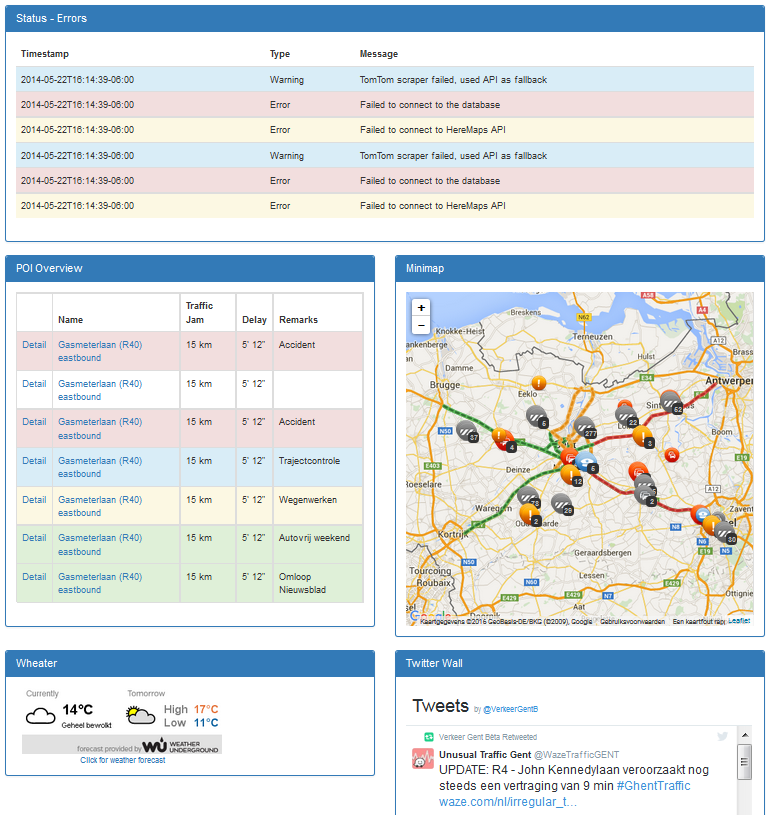
\includegraphics[width=0.6\textwidth]{images/dashboard.png}\\
\caption{Handleiding - Dashboard}
\end{figure}

Om verder te gaan naar de detail pagina’s kunt u gebruik maken van de links aan de bovenkant van de pagina.
Zo is het mogelijk om een overzicht te krijgen van de verschillende routes in de stad Gent. Ook een weergave op kaart en vergelijking tussen verschillende routes is mogelijk.

\subsection{Overview}

Bovenaan de pagina \textbf{“Overview”} kan u kiezen uit de tabbladen: \textbf{“Summary”} , \textbf{“For each provider”} en “By route”.

\begin{figure}[H]
\centering
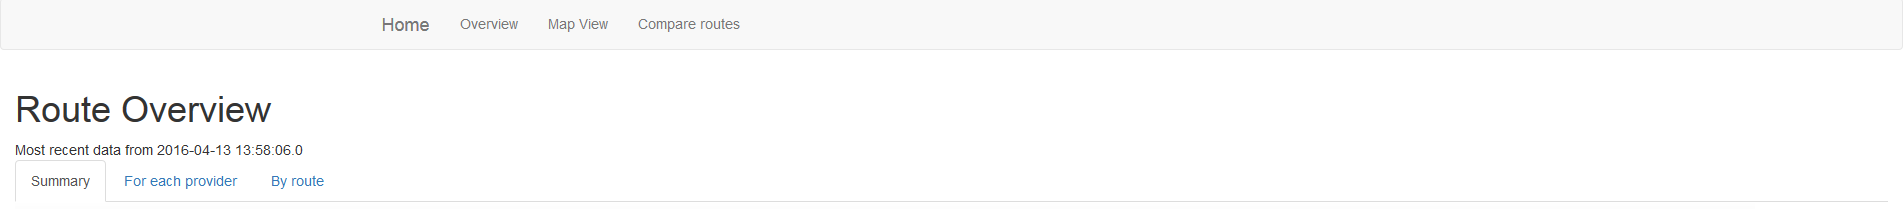
\includegraphics[width=\textwidth]{images/overview.png}\\
\caption{Handleiding - Overview}
\end{figure}

\subsubsection{Summary}

Het tabblad “Summary” geeft een samenvatting van de verschillende routes in beide richtingen. De belangrijkste data zoals naam (Name), afstand (Distance), standaard reisduur (Standard Travel Time), huidige tijdsduur (Current Travel Time) en vertraging (Delay) worden weergeven. Het is mogelijk te sorteren op een bepaald onderwerp door op de hoofding van de tabel te klikken. 

Afhankelijk van de opgelopen vertraging wordt een kleur toegekend aan elk traject. De kleur aanduiding varieert tussen groen (geen file) en rood (zware file).

De trajecten worden in beide richtingen weergeven. Dit wordt aangegeven door de windrichting waarin deze gelegen zijn. (East - West - North - South bound). Bij het klikken op een traject komt u terecht op de detail pagina voor dat traject.


\begin{figure}[H]
\centering
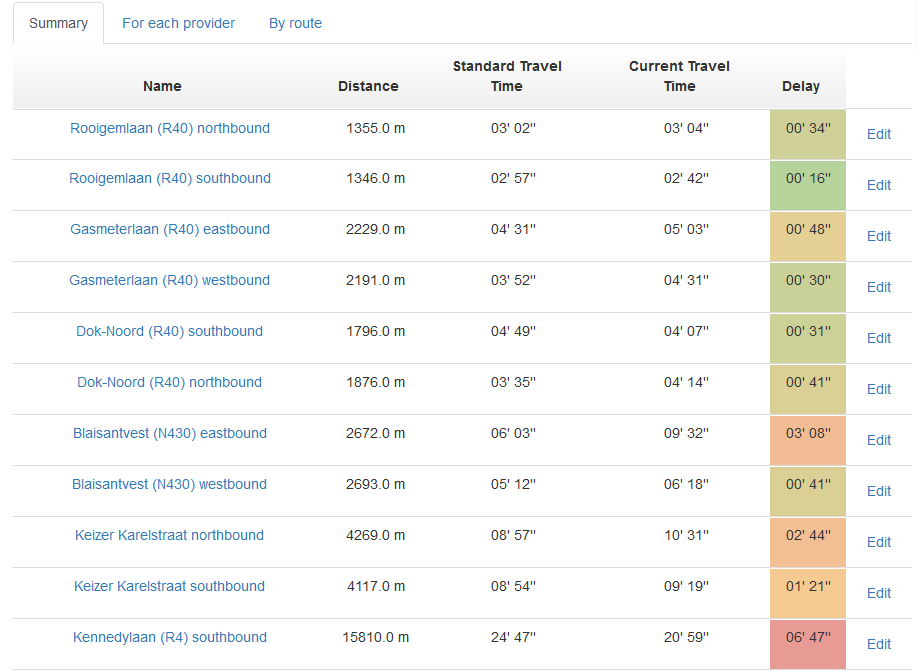
\includegraphics[width=0.75\textwidth]{images/summary.png}\\
\caption{Handleiding - Summary}
\end{figure}

Wijzigingen aan de routes kunnen gemaakt worden door bij een bepaalde route op Edit te klikken. Dit wordt hieronder verder beschreven.

\begin{figure}[H]
\centering
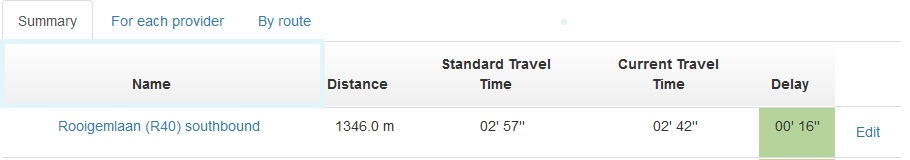
\includegraphics[width=0.75\textwidth]{images/edit.png}\\
\caption{Handleiding - Zoom in op Edit}
\end{figure}

\subsubsection{Detail per traject}

Op deze pagina vindt u de gedetailleerde informatie over het gekozen traject. 

\begin{itemize} 
\item Bovenaan worden de reistijden en vertragingen per provider weergeven. Aan de rechterkant staat het traject afgebeeld op een kaart met een visuele weergave van hoe het verkeer verloopt op dit traject.
\item Bij \textbf{Filteroptions} kan de begin- en einddatum geselecteerd worden als parameters voor het genereren van een grafiek. 
\item In \textbf{History} wordt de grafiek gegenereerd die de tijdsduur, om dit traject af te leggen, grafisch voorstelt tussen het interval ingesteld bij filteroptions.
\item \textbf{Traffic jams} geeft alle files die zijn opgevangen in dat bepaald interval. Zo wordt er weergeven hoe lang de file heeft geduurd (\textbf{Duration}), wat de gemiddelde vertraging (\textbf{Avg delay}) en piek vertraging (\textbf{Peak delay}) was en de mogelijke oorzaken (\textbf{Possible causes}) van de file. De mogelijke oorzaken kunnen invloeden zijn van ongevallen, werken of het weer.
\end{itemize}

\begin{figure}[H]
\centering
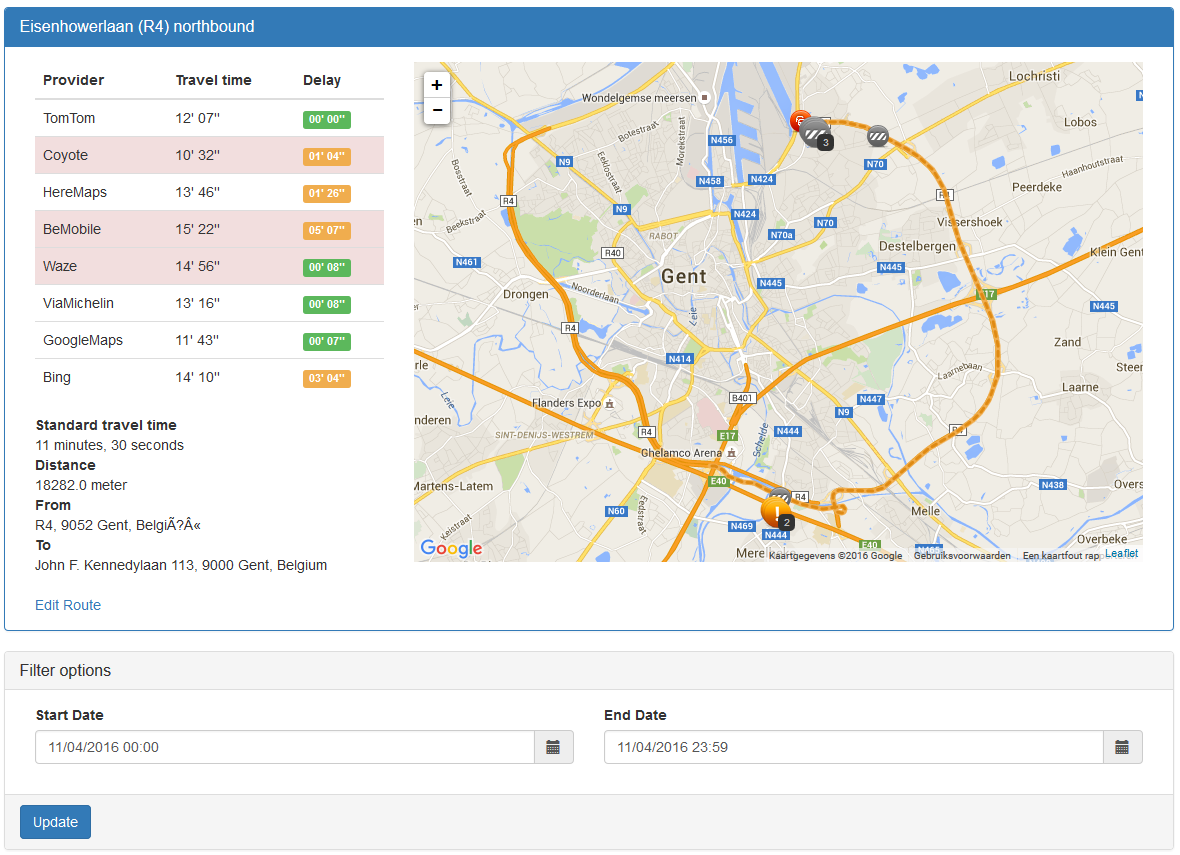
\includegraphics[width=0.75\textwidth]{images/detail.png}\\
\caption{Handleiding - Detail (1/2)}
\end{figure}

\begin{figure}[H]
\centering
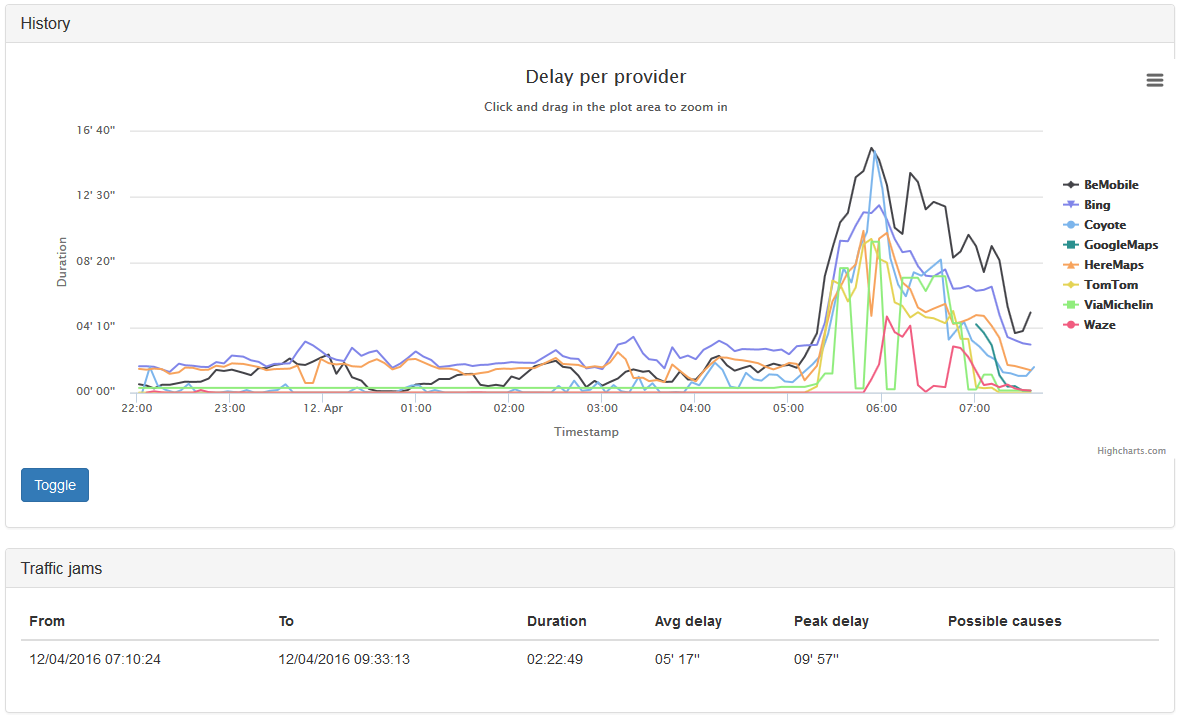
\includegraphics[width=0.75\textwidth]{images/detail2.png}\\
\caption{Handleiding - Detail (2/2)}
\end{figure}

\subsubsection{Edit}

Op het tabblad \textbf{"Summary"} kunnen de trajecten aangepast worden via de knop \textbf{Edit}. Hier kunnen de \textbf{name}, \textbf{from}- en \textbf{to} positions van het traject aangepast worden. De start- en eindpositie kunnen op 2 manieren aangepast worden, door de positie in te geven in het tekstveld of door op het kaartje de rode pijl te verslepen via de rechtermuisknop. Klik na de aanpassingen onderaan op \textbf{Save}.

\begin{figure}[H]
\centering
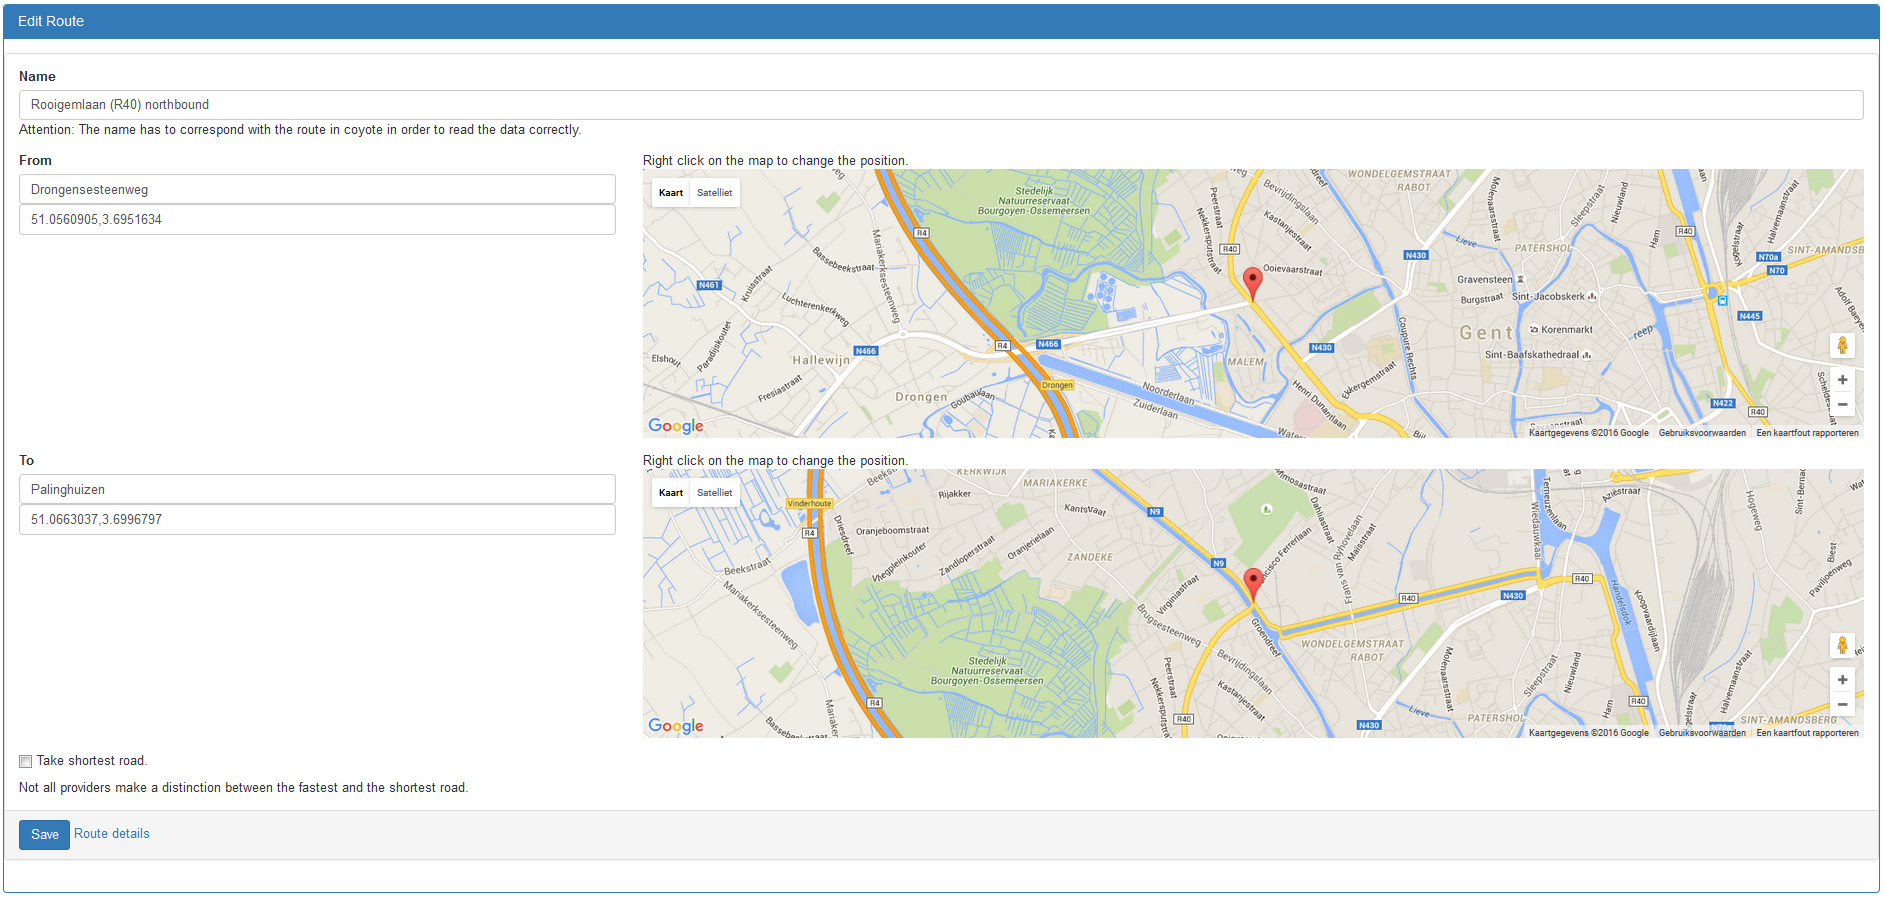
\includegraphics[width=0.75\textwidth]{images/editRoute.png}\\
\caption{Handleiding - Aanpassen Route}
\end{figure}

\subsubsection{For each provider}

Op het tabblad \textbf{“For each provider”} worden de reistijd (\textbf{CTT, Current Travel Time}) en de vertraging (\textbf{D, Delay}) per traject en per verkeersprovider weergegeven. Via het tandwiel kan er worden om bepaalde providers tijdelijk uit te schakelen in het overzicht.

\textbf{Betekenis van de kolommen}
\begin{itemize} 
\item \textbf{Distance} geeft de afstand van het traject.
\item \textbf{Current Travel Time} wordt berekend door het gemiddelde te nemen over de huidige reistijden van de verschillende providers.
\item \textbf{Avg. Delay} geeft de gemiddelde vertraging voor alle providers.
\item \textbf{CCT} geeft de huidige reistijd per provider weer.
\item \textbf{D}  geeft de huidige vertraging per provider weer.
\end{itemize}

\begin{figure}[H]
\centering
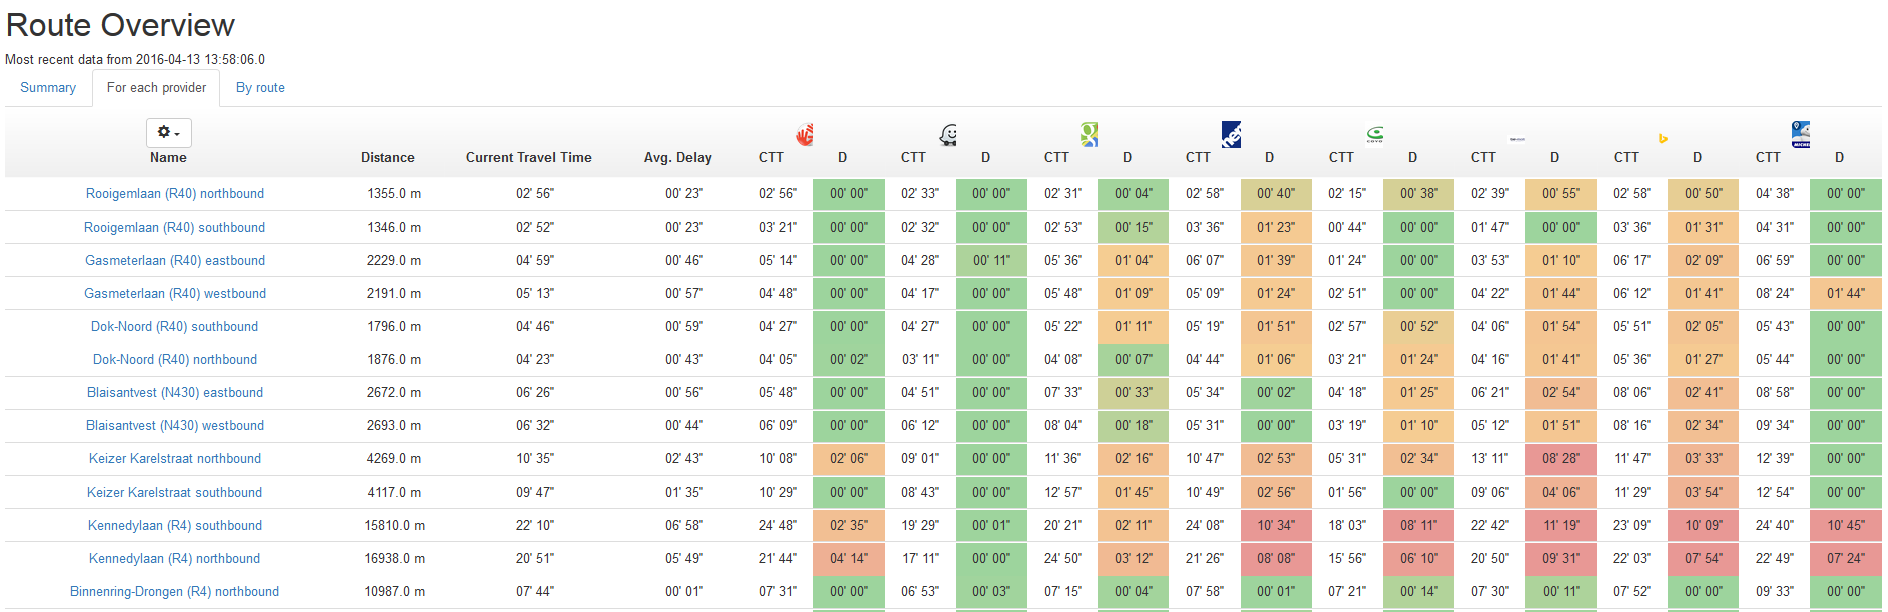
\includegraphics[width=\textwidth]{images/forEachProvider.png}\\
\caption{Handleiding - For Each Provider}
\end{figure}

\subsubsection{By Route}

Op het tabblad “By route” word dezelfde data weergeven zoals bij “For each provider”, maar hier wordt de data gesorteerd per route.

\begin{figure}[H]
\centering
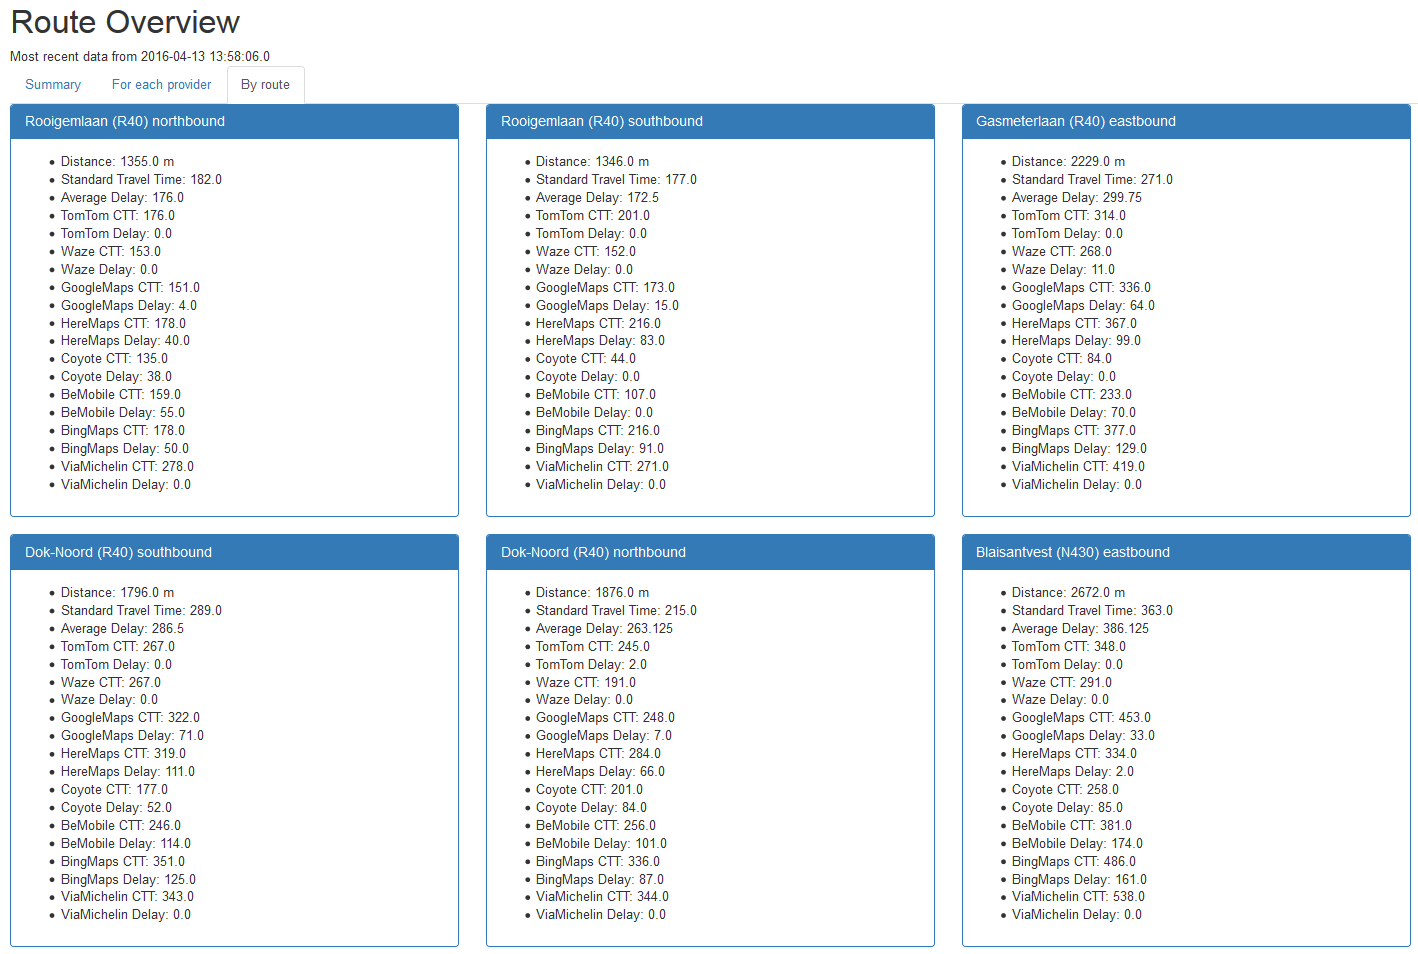
\includegraphics[width=0.9\textwidth]{images/byRoute.png}\\
\caption{Handleiding - By Route}
\end{figure}

\subsection{Map View}

Op de pagina \textbf{“Map View”} worden alle trajecten afgebeeld op een kaart. Afhankelijk van de opgelopen vertraging wordt een kleur toegekend aan elk traject. Het traject wordt aangeduid met een bewegende route waardoor het duidelijk wordt in welke richting het verkeer zich beweegt. Door een traject af te vinken wordt het niet meer weergegeven op de kaart.

\begin{figure}[H]
\centering
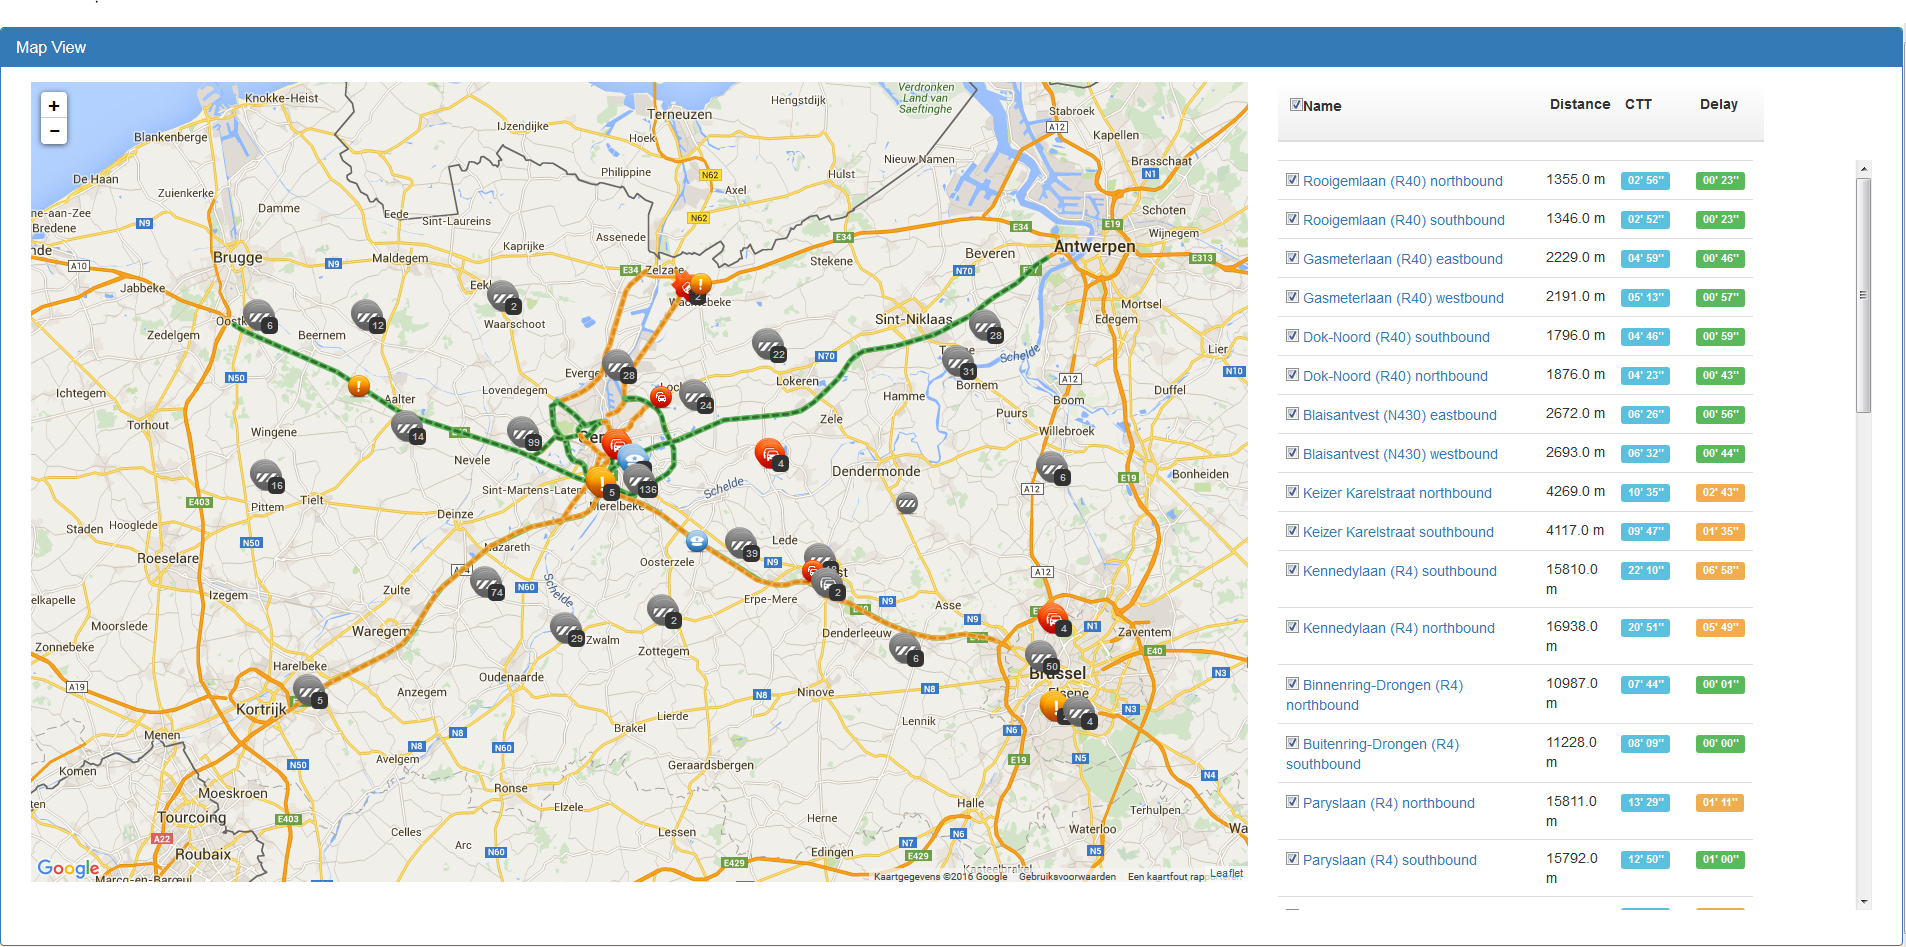
\includegraphics[width=\textwidth]{images/mapView.png}\\
\caption{Handleiding - Map View}
\end{figure}